% \documentclass{article}

% % Language setting
% % Replace `english' with e.g. `spanish' to change the document language
% \usepackage[english]{babel}

% % Set page size and margins
% % Replace `letterpaper' with`a4paper' for UK/EU standard size
% \usepackage[letterpaper,top=2cm,bottom=2cm,left=3cm,right=3cm,marginparwidth=1.75cm]{geometry}

% % Useful packages
% \usepackage{amsmath}
% \usepackage{amssymb}
% \usepackage{mathtools}
% \usepackage{graphicx}
% \usepackage{enumitem}
% \usepackage[colorlinks=true, allcolors=blue]{hyperref}

% \usepackage{hyperref}
% \hypersetup{
%     colorlinks=true,
%     linkcolor=blue,
%     filecolor=magenta,      
%     urlcolor=cyan,
%     pdftitle={Overleaf Example},
%     pdfpagemode=FullScreen,
%     }

% \urlstyle{same}

% \usepackage{tikz-cd}

% %%%%%%%%%%% Box pacakges and definitions %%%%%%%%%%%%%%
% \usepackage[most]{tcolorbox}
% \usepackage{xcolor}
% \usepackage{csquotes}


% % Define the colors
% \definecolor{boxheader}{RGB}{0, 51, 102}  % Dark blue
% \definecolor{boxfill}{RGB}{173, 216, 230}  % Light blue

% % Define the tcolorbox environment
% \newtcolorbox{mathdefinitionbox}[2][]{%
%     colback=boxfill,   % Background color
%     colframe=boxheader, % Border color
%     fonttitle=\bfseries, % Bold title
%     coltitle=white,     % Title text color
%     title={#2},         % Title text
%     enhanced,           % Enable advanced features
%     attach boxed title to top left={yshift=-\tcboxedtitleheight/2}, % Center title
%     boxrule=0.5mm,      % Border width
%     sharp corners,      % Sharp corners for the box
%     #1                  % Additional options
% }
% %%%%%%%%%%%%%%%%%%%%%%%%%

% \newtcolorbox{dottedbox}[1][]{%
%     colback=white,    % Background color
%     colframe=white,    % Border color (to be overridden by dashrule)
%     sharp corners,     % Sharp corners for the box
%     boxrule=0pt,       % No actual border, as it will be drawn with dashrule
%     boxsep=5pt,        % Padding inside the box
%     enhanced,          % Enable advanced features
%     overlay={\draw[dashed, thin, black, dash pattern=on \pgflinewidth off \pgflinewidth, line cap=rect] (frame.south west) rectangle (frame.north east);}, % Dotted line
%     #1                 % Additional options
% }

% \usepackage{biblatex}
% \addbibresource{sample.bib}


% %%%%%%%%%%% New Commands %%%%%%%%%%%%%%
% \newcommand*{\T}{\mathcal T}
% \newcommand*{\cl}{\text cl}


% \newcommand{\ket}[1]{|#1 \rangle}
% \newcommand{\bra}[1]{\langle #1|}
% \newcommand{\inner}[2]{\langle #1 | #2 \rangle}
% % \newcommand{\mean}[1]{\langle #1 \rangle}
% \newcommand{\R}{\mathbb{R}}
% \newcommand{\C}{\mathbb{C}}
% \newcommand{\V}{\mathbb{V}}
% \newcommand{\Hilbert}{\mathcal{H}}
% \newcommand{\oper}{\hat{\Omega}}
% \newcommand{\lam}{\hat{\Lambda}}
% \newcommand{\defeq}{\vcentcolon=}
% \newcommand{\}{\vcentcolon=}
% \newcommand{\bigslant}[2]{{\raisebox{.2em}{$#1$}\left/\raisebox{-.2em}{$#2$}\right.}}
% \newcommand{\restr}[2]{{% we make the whole thing an ordinary symbol
%   \left.\kern-\nulldelimiterspace % automatically resize the bar with \right
%   #1 % the function
%   \vphantom{\big|} % pretend it's a little taller at normal size
%   \right|_{#2} % this is the delimiter
%   }}
% %%%%%%%%%%%%%%%%%%%%%%%%%%%%%%%%%%%%%%%


% \tcbset{theostyle/.style={
%     enhanced,
%     sharp corners,
%     attach boxed title to top left={
%       xshift=-1mm,
%       yshift=-4mm,
%       yshifttext=-1mm
%     },
%     top=1.5ex,
%     colback=white,
%     colframe=blue!75!black,
%     fonttitle=\bfseries,
%     boxed title style={
%       sharp corners,
%     size=small,
%     colback=blue!75!black,
%     colframe=blue!75!black,
%   } 
% }}

% \newtcbtheorem[number within=section]{Theorem}{Theorem}{%
%   theostyle
% }{thm}

% \newtcbtheorem[number within=section]{Definition}{Definition}{%
%   theostyle
% }{def}


%%%%%%%%%%%%%%%%%%%%%%%%%%% IMPORTED FROM MATH 214 NOTES %%%%%%
\documentclass{article}

% Language setting
% Replace `english' with e.g. `spanish' to change the document language
\usepackage[english]{babel}

% Set page size and margins
% Replace `letterpaper' with`a4paper' for UK/EU standard size
\usepackage[letterpaper,top=2cm,bottom=2cm,left=3cm,right=3cm,marginparwidth=1.75cm]{geometry}

% Useful packages
\usepackage{amsmath}
\usepackage{amssymb}
\usepackage{mathtools}
\usepackage{graphicx}
\usepackage{enumitem}
\usepackage[colorlinks=true, allcolors=blue]{hyperref}

\usepackage{hyperref}
\hypersetup{
    colorlinks=true,
    linkcolor=blue,
    filecolor=magenta,      
    urlcolor=cyan,
    pdftitle={Math 214 HW 4},
    pdfpagemode=FullScreen,
    }

\urlstyle{same}

\usepackage{tikz-cd}

%%%%%%%%%%% Box pacakges and definitions %%%%%%%%%%%%%%
\usepackage[most]{tcolorbox}
\usepackage{xcolor}

% Define the colors
\definecolor{boxheader}{RGB}{0, 51, 102}  % Dark blue
\definecolor{boxfill}{RGB}{173, 216, 230}  % Light blue

% Define the tcolorbox environment
\newtcolorbox{mathdefinitionbox}[2][]{%
    colback=boxfill,   % Background color
    colframe=boxheader, % Border color
    fonttitle=\bfseries, % Bold title
    coltitle=white,     % Title text color
    title={#2},         % Title text
    enhanced,           % Enable advanced features
    attach boxed title to top left={yshift=-\tcboxedtitleheight/2}, % Center title
    boxrule=0.5mm,      % Border width
    sharp corners,      % Sharp corners for the box
    #1                  % Additional options
}
%%%%%%%%%%%%%%%%%%%%%%%%%

\newtcolorbox{dottedbox}[1][]{%
    colback=white,    % Background color
    colframe=white,    % Border color (to be overridden by dashrule)
    sharp corners,     % Sharp corners for the box
    boxrule=0pt,       % No actual border, as it will be drawn with dashrule
    boxsep=5pt,        % Padding inside the box
    enhanced,          % Enable advanced features
    overlay={\draw[dashed, thin, black, dash pattern=on \pgflinewidth off \pgflinewidth, line cap=rect] (frame.south west) rectangle (frame.north east);}, % Dotted line
    #1                 % Additional options
}

\usepackage{biblatex}
\addbibresource{sample.bib}


%%%%%%%%%%% New Commands %%%%%%%%%%%%%%
\newcommand*{\T}{\mathcal T}
\newcommand*{\cl}{\text cl}
\newcommand{\bP}{\mathbb{P}}
\newcommand{\bS}{\mathbb{S}}


\newcommand{\ket}[1]{|#1 \rangle}
\newcommand{\bra}[1]{\langle #1|}
\newcommand{\inner}[2]{\langle #1 | #2 \rangle}
\newcommand{\R}{\mathbb{R}}
\newcommand{\C}{\mathbb{C}}
\newcommand{\A}{\mathbb{A}}
\newcommand{\sphere}{\mathbb{S}}
\newcommand{\V}{\mathbb{V}}
\newcommand{\Hilbert}{\mathcal{H}}
\newcommand{\oper}{\hat{\Omega}}
\newcommand{\lam}{\hat{\Lambda}}
\newcommand{\defeq}{\vcentcolon=}

\newcommand{\bigslant}[2]{{\raisebox{.2em}{$#1$}\left/\raisebox{-.2em}{$#2$}\right.}}
\newcommand{\restr}[2]{{% we make the whole thing an ordinary symbol
  \left.\kern-\nulldelimiterspace % automatically resize the bar with \right
  #1 % the function
  \vphantom{\big|} % pretend it's a little taller at normal size
  \right|_{#2} % this is the delimiter
  }}
%%%%%%%%%%%%%%%%%%%%%%%%%%%%%%%%%%%%%%%


\tcbset{theostyle/.style={
    enhanced,
    sharp corners,
    attach boxed title to top left={
      xshift=-1mm,
      yshift=-4mm,
      yshifttext=-1mm
    },
    top=1.5ex,
    colback=white,
    colframe=blue!75!black,
    fonttitle=\bfseries,
    boxed title style={
      sharp corners,
    size=small,
    colback=blue!75!black,
    colframe=blue!75!black,
  } 
}}

\newtcbtheorem[number within=section]{Theorem}{Theorem}{%
  theostyle
}{thm}

\newtcbtheorem[number within=section]{Definition}{Definition}{%
  theostyle
}{def}


%%%%%%%%%%%%%%%%%%%%%%%%%%%%%%%%%%%%%%%%%%%%%%%%%%%%%


\title{Physics 198 Notes}
\author{Keshav Balwant Deoskar}

\begin{document}
\maketitle

% \vskip 0.5cm
These are notes taken from lectures on Topology, Geometry, and Algebra delivered by EVibhu Ravindran, Pablo Castano, and Michelle Dong for UC Berekley's Physics 198 class (DeCal) in the Sprng 2024 semester. Any errors that may have crept in are solely my fault.
% \pagebreak 

\tableofcontents

\pagebreak

%%%%%%%%%%%%%%%%%%%%%%%%%%%%%%%%%%%%%%%%%%%%%%%%%%%%%%%%%%%%%%%%%%
\section{January 23 - Classical Mechanics Review, Linear Algebra}
%%%%%%%%%%%%%%%%%%%%%%%%%%%%%%%%%%%%%%%%%%%%%%%%%%%%%%%%%%%%%%%%%
Classical mechanics is the field of physics everyone first encounters, and usually this only extends to \textbf{Newtonian Mechanics}.

\begin{align*}
  &\textbf{Newtonian Mechanics} \\
  & F = ma \\
  & E = K + V
\end{align*}

\vskip 1cm
Newtonian Mechanics is powerful, but it is a local theory. One has to use the second law at each point in time to study the behavior of a system. For some problems, it's easier to work with the equivalent, but \textbf{global} formulations of classical mechanics, which are \textbf{Lagrangian} and \textbf{Hamiltonian} mechanics.

\begin{align*}
  &\textbf{Lagrangian}\\
  &L = K - V \\
  &\text{S.H.O. } = \frac{1}{2}m\dot{x}^2 - \frac{1}{2}kx^2\\
  &\text{Action: } S = \int dt L = \int dt d^3x \mathcal{L}\\
  &\text{Euler Lagrange Equations: } \frac{\partial L}{\partial x} - \frac{d}{dt} \left( \frac{\partial L}{\partial (\partial_t x)} \right) = 0 \\
  \vdots
\end{align*}

*** Show equivalence of Euler-Lagrange Equations and Netwon's 2nd Law.

\vskip 1cm
Hamiltonian Mechanics has the same global structure as Lagrangian Mechanics, but is useful because it makes it easier to spot symmetries and conserved quantities. The Hamiltonian $H$ is obtained from the Lagrangian $L$ by a \textbf{Legendre Transformation}.

\begin{align*}
  &\textbf{Hamiltonian} \\
  &\text{Write equations later.}
\end{align*}

\vskip 1cm
*** Be sure to explain conjugate momentum, phase/configuration space, Hamiltons Equations. 

\vskip 1cm
\subsection{Linear Algebra}

Linearly Algebra is a remarkably powerful branch of math because of how many different systems can be modelled using vector spaces. Familiar examples of vector spaces are $\R$, $\C$, and in fact $\R^n$ and $\C^n$, but we'll see some wild examples later.

\subsubsection{Vector Spaces}

\begin{dottedbox}
  \underline{\textbf{Vector Space:}} A set $V$ with some sense of addition and multiplication is said to be a vector space if its operations satify
  \begin{itemize}
    \item \textbf{Commutativity:} $u + v = v + u, \forall u, v \in V$
    \item \textbf{Associativity:} $(u + v) + w = u + (v + w), \forall u,v,w \in V$
    \item \textbf{Additive Identity:}
    \item \textbf{Additive Inverse:}
    \item write the rest of the vector space properties.
  \end{itemize}
\end{dottedbox}

\vskip 1cm

\subsubsection{Subspaces}
A subset $U$ of $V$ is called a \textbf{subspace} of $V$ if $U$ is itself a vector space.

\vskip 1cm
\subsubsection{Linear Map}
Given Definition

\vskip 1cm
Some spaces associated with a Linear Map are the \textbf{Kernal} and \textbf{Image}. 

\begin{dottedbox}
  For a linear map $T : V \rightarrow W$, 
  \begin{itemize}
    \item The \underline{\textbf{Kernal of T}} is defined as 
    \[ \ker(T) = \{ v \in V : Tv = 0 \}  \]

    \item The \underline{\textbf{Image of T}} is defined as 
    \[ \text{Im}(T) = \{ w \in W : w = Tv \text{ for some } v \in V \} \]
  \end{itemize}
\end{dottedbox}

[Include diagram or something to make this not dry]

\subsubsection{Injectivity, Surjectivity, etc.}
Write about when a linear map is injective, surjective etc.

\subsubsection{Linear Functionals, Inner Products}
Talk about linear functionals (aka dual vectors aka covectors) and inner Products

\underline{Exercise:} Find an example of an infinite dimensional vector space which is not isomorphic to its dual.

\vskip 1cm
\subsubsection{Spectral Theorem for Self-Adjoint Operators}

\vskip 1cm
\subsubsection{Tensors}
An $(r, s)-$Tensor $T$ is a multi-linear map 
\[ T : \underbrace{V^{*} \times \cdots \times V^{*}}_{r} \times \underbrace{V \times \cdots \times V}_s \rightarrow \mathbb{F} \]


% \vskip 1cm
\pagebreak
\section{January 25 - Algebra, Group Theory}

\vskip 1cm
\subsection{Revisiting vector spaces, duals, and tensors}
Last time, we defined the set of linear maps between vector spaces $V, W$ and denoted it as $\mathcal{L}(V, W)$.

\vskip 1cm
\begin{dottedbox}
  The set of linear maps $\mathcal{L}(V, W)$ is itself a vector space with addition and scalar multiplication defined as : 
  \begin{align*}
    Addition&: (T+S)(v) \defeq T(v) + S(v)\\
    Multiplication&: (\lambda T)(v) \defeq \lambda \cdot (T(v)) 
  \end{align*}
  where $T, S \in \mathcal{L}(V, W)$, $\lambda \in \mathbb{F}, v \in V$. 
\end{dottedbox}

\vskip 1cm
\underline{\textbf{Note:}} If $V$ is a vector space over the field $\mathbb{F}$, another name for $\mathcal{L}(V, \mathbb{F})$ is the \textbf{Dual Space, $\mathbf{V^{\star}}$}.


Also, last time we saw the formal definition of a tensor, but we didn't see a concete example.
\vskip 1cm
\begin{dottedbox}
  \underline{Example:} For an example of a physical tensor, we can consider the Lagrangian of a free (classical) particle:
  \begin{align*}
    L &= T - V \\
    &= \sum_{i} \frac{1}{2} m \dot{x}^2 \\
    &= \sum_{i} \frac{1}{2} m \delta_{ij} \dot{x}^i \dot{x}^j
  \end{align*}
  and this describes the motion in flat space. However, in curved space (eg. space-time) we can take the influence of the curvature into account by replacing $\delta_{ij}$ with $g_{ij}$ where $g_{ij}$ depends only on tim i.e.

  \[ \boxed{L = \sum_{i} \frac{1}{2} m g_{ij} \dot{x}^i \dot{x}^j} \]

  \vskip 1cm
  Solving the Euler-Lagrange equations, we have 
  \begin{align*}
    \frac{\partial L}{\partial x^i} - \frac{d}{dt}\left( \frac{\partial L}{\partial \dot{x^i}} \right) &= 0 \\
    \implies \frac{1}{2} m \frac{\partial g_{ik}}{\partial x^i}x^j x^k - \frac{d}{dt} \left( m g_{ij} x^i x^j \right) &= 0 \\
    \implies \text{Complete this example later}&
  \end{align*}  
\end{dottedbox}

\vskip 1cm
\subsection{Group Theory}

\vskip 0.5cm
Now that we've covered that stuff, we move onto some \textbf{group theory}. This branch of math is essentially the study of \textbf{symmetries} i.e. transformations that leave a system unchanged or \textbf{invariant}.

\vskip 0.5cm
\begin{mathdefinitionbox}{Formal definition of a Group}
  \vskip 0.5cm
  A group is a pair $(G, \star)$, where $G$ is a set and $\star : G \rightarrow G$ is a \emph{bilinear operation}, satifying three properties. Namely, 
  \begin{enumerate}[label=(\alph*)]
    \item Associativity: $a \star ( b \star c) = (a \star b) \star c$ 
    
    \item Identity: There exsits an element $e \in G$ such that, for all $g \in G$,
    \[ g \star e = e \star g = g \]

    \item Inverses: For each $a \in G$, there must exist an \emph{inverse} element denoted $a^{-1}$ such that 
    \[ a \star a^{-1} = a^{-1} \star a \]
  \end{enumerate}
\end{mathdefinitionbox}

\vskip 0.5cm
For example,
\begin{itemize}
  \item Any vector space $V$ with vector addition being the bilinear product $\star$ is a group.
  \item The set of permutations of three objects, called the \textbf{Symmetric group of order 3}, denoted $S_3$ is a group.
\end{itemize}

\vskip 0.5cm
Note that in a vector space, $v \star w = w \star v$. This is a very special property called \textbf{commutativity} i.e. the order in which we operate group elements does not matter. Such a group is said to be \textbf{commutative} or \textbf{abelian}. In constrast to this, the symmetric group of order 3, $S_3$ is \textbf{non-abelian} (in fact, it's the smallest such group!)

\vskip 0.5cm
\underline{\textbf{Note:}} The number of elements in a group $G$ is called its \emph{order} and is denoted by $\lvert G \rvert$.

\vskip 1cm
\subsubsection{Subgroup}

\vskip 0.5cm
\begin{mathdefinitionbox}{Subgroup}
  \vskip 0.5cm
  \begin{itemize}
    \item   For a group $G$, a subset $H \subset G$ is called a subgroup if 
    \begin{enumerate}[label=(\alph*)]
      \item $e \in H$
      \item $a, b \in H \implies ab \in H$ (this is called \emph{closure})
      \item $a \in H \implies a^{-1} \in H$ 
    \end{enumerate}

    \item If $H$ is a subgroup of $G$, we write $H \leq G$.
  \end{itemize}
\end{mathdefinitionbox}



\vskip 1cm
\subsubsection{Coset}

\vskip 0.5cm
\begin{mathdefinitionbox}{Coset}
\vskip 0.5cm
  \begin{itemize}
    \item For a group $G$ and subgroup $H \subset G$, we can consider an element $g \in G, g \not\in H$ and define the \emph{left coset of $H$} to be
    \[ gH \defeq \{ gh : h \in H \} \]

    \item There is a one to one correspondence between a subgroup $H$ and any coset of $H$.
  \end{itemize}
\end{mathdefinitionbox}

\vskip 1cm
\subsubsection{Lagrange's Theorem}

\vskip 0.5cm
\begin{dottedbox}
  \underline{\textbf{Theorem:}} If $G$ is a finite group and $H \subset G$ is a subgroup, then $H$ divides $G$.

  \vskip 0.5cm
  \underline{\textbf{Proof Sketch:}} Let's define the equvalence relation $g_1 \sim g_2$ iff $g_1^{-1} g_2 \in H$. Suppose 
  \[ g_2 H = g_1 H \]
  Then 
  \[ g_1^{-1}g_2 H = H \]
  
  Any two distinct cosets are disjoint, thus all cosets are of equal order since they are disjoint equivalence classes. So, 
  \begin{align}
    \lvert G \rvert &= |g_1 H| + |g_2 H| + c\dots \\
    &= \underbrace{k}_{\# of cosets} \cdot \lvert H \rvert
  \end{align}

  Thus, $\lvert H \rvert$ divides $\lvert G \rvert$.
\end{dottedbox}

\vskip 1cm
\subsubsection{Normal subgroups}

\vskip 0.5cm
Some subgroups have the very special propert that their \emph{left and right cosets are equal}. This is unusual since group element multiplication is not generally guaranteed to be commutative.

\begin{mathdefinitionbox}{Normal Subgroup}
\vskip 0.5cm
  A subset of a group $G$ is said to be a \textbf{normal subgroup} if 
  \begin{itemize}
    \item It is a subgroup
    \item $gN = Ng$ 
  \end{itemize}
  A subgroup is denoted as $N \trianglelefteq G$.
\end{mathdefinitionbox}

\vskip 0.5cm
Normal subgroups allow us to produce a very important class of groups called \emph{Quotient Groups}.

\vskip 1cm
\subsubsection{Quotient Groups}

\vskip 0.5cm

\begin{mathdefinitionbox}{Quotient Group}
\vskip 0.5cm
  Given a group $G$ and normal subgroup $N \trianglelefteq G$, we can define the \textbf{quotient group} as 
  \[ G/N \defeq \{ [a] = aN : a \in G \} \]
\end{mathdefinitionbox}

\vskip 0.5cm

\begin{dottedbox}
\underline{\textbf{Exercise:}} Verify that the bilinear product on the quotient group
\[ [a] \star [b] = [a b] \]
is \textbf{well defined} i.e. does not depend on the specific elements $a, b$ chosen to represent the equivalence classes $[a], [b]$.
\end{dottedbox}

\vskip 1cm
\subsection{Group Homomorphisms}
\vskip 0.5cm
So far we've spoken about a group and its subgroups, all stuff that was relatively self-contained. However, in math, we often want to study \emph{maps between objects}. The "natural" map between groups is called a \emph{homomorphism}.

\vskip 0.5cm
Now, the numbers $1$ to $10$ in english are "One", "Two", ...,"Ten" whereas in say Spanish they are "Unos", "Dos", ..., "Diez". Furthermore, to convey the idea of adding numbers in English, we can say "One \textbf{plus} Two" whereas the same idea in Spanish would be "Uno más Dos".

\vskip 0.5cm
Clearly the numbers 1 to 10 are the same regardless of the names we use to describe them in different languages, and similarly for the process of adding them (which is a \emph{really} just a bilinear product). So, there is a sort of mapping between the two.

\vskip 0.5cm
Drawing from this (imperfect) analogy, a homomorphism between two groups is a like a dictionary, which maps the words between the two languages and allows us to translate. 

\vskip 0.5cm
\begin{mathdefinitionbox}{Group Homomorphisms and Isomorphisms}
\vskip 0.5cm
\begin{itemize}
  \item For groups $(G, \cdot)$ and $(H, \star)$, a map $\phi : G \rightarrow H$ is a homeomorphism if 
  \[ \phi(a \cdot b) = \phi(a) \star \phi(b) \]

  \item Further, if the map if \emph{bijective} then it is called an \textbf{Isomorphism.} We then say $G$ and $H$ are isomorphic, denoted as $G \cong H$.
\end{itemize}
\end{mathdefinitionbox}

\vskip 0.5cm
\begin{dottedbox}
\begin{itemize}
  \item   For example, a group $G$ is isomorphic to \emph{itself}. The map $G \rightarrow G$ is then called an \textbf{ automorphism} 
  
  \item An \textbf{inner automorphism} is of the form 
  \[ \phi_h(g) = h^{-1}gh \]
  i.e. it conjugates each element $g \in G$ with respect to some particular $h \in G$.
\end{itemize}
\end{dottedbox}

\vskip 0.5cm
Group Homomorphisms are \emph{structure preserving}.


\vskip 1cm
\subsection{Kernel, Image, and the First Isomorphism Theorem:}

Similar to vector spaces, we define the \emph{Kernel} and \emph{image} of a map $\phi : G \rightarrow H$ to be 
\begin{align*}
  &\text{Ker}(\phi) \defeq \{ g \in G : \phi(g) = e \} \\
  &\text{Im}(\phi) \defeq \{ h \in H : h = \phi(g), g \in G \} 
\end{align*}

Then, the first isomorphism theorem is as follows:

\vskip 0.5cm
\begin{dottedbox}
  \underline{\textbf{First Isomorphism Theorem:}} For groups $G, H$ and map $\phi : G \rightarrow H$
  \begin{enumerate}[label=(\alph*)]
    \item Ker$(\phi)$ is a normal subgroup of $G$ i.e. Ker$(\phi) \trianglelefteq G$.
    \item Im$(\phi)$ is a subgroup of $H$ i.e. Im$(\phi) \leq H$.
    \item The quotient of $G$ by ker$(\phi)$ is isomorphic to Im$(\phi)$ i.e.
    \[ G / \text{Ker}(\phi) \cong \text{Im}(\phi) \]
  \end{enumerate}
\end{dottedbox}

\vskip 1cm
\subsection{Fundamental Group}

Consider a donut shaped surface called a \emph{Torus}, denoted $T$, and some point $p \in T$ [Complete this later].

\pagebreak
\section{January 30 - Point set Topology}

\vskip 0.5cm
\subsection{What is a Topological Space?}

\begin{mathdefinitionbox}{Topologcal Space}
  \begin{itemize}
    \item A topology is a pair $(M, \mathcal{O})$ where $M$ is some arbitrary set and $\mathcal{O}$ is a collection of subsets of $M$ i.e. $\mathcal{O} \subset \mathcal{P}(M)$ such that 
    \begin{itemize}
      \item $\emptyset, M \in \mathcal{O}$
      \item Finite intersections of sets already in $\mathcal{O}$ are also in $\mathcal{O}$: $\{ U, V \} \subset \mathcal{O} \implies \bigcap \{ U, V\} \subset \mathcal{O}$ 
      \item Arbitrary unions of sets already in $\mathcal{O}$ are also in $\mathcal{O}$:$C \subseteq \mathcal{O} \implies \bigcup C \subseteq \mathcal{O}$ 
    \end{itemize}
  \end{itemize}
\end{mathdefinitionbox}

\vskip 0.5cm
\begin{dottedbox}
  Examples:
  \begin{itemize}
    \item Let $M$ be a set. Then, $\mathcal{O} = \{\emptyset, M\}$ is called the \emph{chaotic topology} on $M$.
    \item Let $\mathcal{O} = \mathcal{P}(M)$ is called the \emph{discrete topology} on $M$.  
  \end{itemize}
\end{dottedbox}

\vskip 0.5cm
\subsubsection*{More goofy ahh adjectives for topologies:}

\begin{dottedbox}
  Let $M$ be a set with two topologies $\tau_1$ and $\tau_2$.
  \begin{itemize}
    \item If $\tau_1 \subset \tau_2$ then $\tau_1$ is \underline{weaker} than $\tau_2$, and equvalently, $\tau_2$ is \underline{stronger} than $\tau_1$.
  \end{itemize}
\end{dottedbox}

\vskip 0.5cm
\subsection{Openness and Closedness}

\vskip 0.5cm
You may have heard of open sets in $\R$, or even $\R^n$. Well, these open sets are actually just the members of the \emph{standard topology on $\R^n$}.

\vskip 0.5cm
In general, "open" just means "member of topology".
\begin{mathdefinitionbox}{Open and closed sets}
  Let $(M, \mathcal{O})$ be a topological space.
  \begin{itemize}
    \item A subset $S \subseteq M$ is \emph{\textbf{open}} (with respect to $\mathcal{O}$) if $S \in \mathcal{O}$.
    \item A subset $U \subseteq M$ is \emph{\textbf{closed}} (with respect to $\mathcal{O}$) if $M \setminus U$ is open.
  \end{itemize}
  Note that "open" does not = "closed"! A set can be \emph{both} open and closed. If we find sufficiently weird spaces, we can even find subsets which are \emph{neither} open or closed! [Include some examples later].
\end{mathdefinitionbox}

\vskip 0.5cm
\subsubsection*{Open balls in $\R^d$}

For instance, the real numbers with the usual metric 
\[ d(x, y) = \sqrt{\sum (y_i - x_i)^2} \]

we can define \emph{\textbf{open ball centered around $x$}} of \textbf{\emph{radius $r$}} to be 

\[ \boxed{ B_r(x) \defeq \{ y \in \R^d \;:\; d(x, y) < r  \} } \]

\vskip 0.5cm
\subsubsection*{Standard Topology on $\R^d$}
We define the standard topology on $\R^d$, $\mathcal{O}_{std}$ by 
\[ U \in \mathcal{O}_{std} \iff \forall p \in U, \; \exists r \in \R^{+} \;:\; B_r(p) \subset U  \]

\vskip 0.5cm
\subsection{Building new topologies out of old ones}
Given one or more topological spaces, there are many ways to combine them/restrict them/quotient them to form new topological spaces.

\vskip 0.5cm
\subsubsection{Subspace Topology}

Given a topological space $(M, \mathcal{O})$ and some subset $N \subset M$, we can turn $N$ into a topological space by endowing it with the \emph{\textbf{subspace topology}} defined as :

\[ \restr{\mathcal{O}}{N} = \{ V \subset M | V = U \cap N \;\text{ for some open set } U \in \mathcal{O}  \} \]

\vskip 0.5cm
\subsubsection{Quotient Topology}
Given a topological space $(M, \mathcal{O})$ and an equivalence relation $\sim$ defined on $M$, we can construct the a new topological space by endowing the \emph{\textbf{quotient set}} with the \emph{\textbf{quotient topology}}:

\begin{align*}
  &\text{Quotient set: } \bigslant{M}{\sim} = \{ [m] \subset \mathcal{P}(M) : m \in M \} \\
  &\text{Quotient topology: } \mathcal{O}_{M / \sim} = \{ U \subset \bigslant{M}{\sim} : \bigcup U = \bigcup_{[a] \in U} [a] \in \mathcal{O}\} 
\end{align*}

\subsubsection*{Examples:}
\begin{itemize}
  \item For example, the standard topology on the unit circle $\mathbb{S}^1$ is [write later]
\end{itemize}

\vskip 0.5cm
\subsubsection{Product Topology}
Given two topological spaces $(A, \mathcal{O}_A)$, $(B, \mathcal{O}_B)$ we can define a topology on $A \times B$ as 
\[ U \in \mathcal{O}_{A \times B} \iff \forall p \in U : \exists (S,T) \in \mathcal{O}_A \times \mathcal{O}_B : S \times T \subseteq U \]

\vskip 0.5cm
\subsection{Sequences and Convergence}

\begin{mathdefinitionbox}{}
  \begin{itemize}
    \item Let $M$ be a set. A sequence in $N$ is a function $q : \mathbb{N} \rightarrow M$.
    \item Let $(M, \mathcal{O})$ be a topological space. A sequence $q$ in $M$ converges \underline{against a limit point} $a \in M$ if $\forall U \in \mathcal{O} : a \in U \implies \exists N : \forall n \geq N : q(n) \in U$.
    \item An open set $U \subseteq M$ such that $a \in U$ is called an \emph{\textbf{open neighborhood}} of $a$ : $U(a)$.
  \end{itemize}
\end{mathdefinitionbox}
% \printbibliography

\begin{mathdefinitionbox}{Continuous maps}
\vskip 0.5cm
  A map $\phi : M \rightarrow N$ between topological spaces $(M, \mathcal{O}_M)$, $(N, \mathcal{O}_N)$ is called \emph{\textbf{continuous}} if for every $S \in \mathcal{O}_n$, the pre-image is open in $M$ i.e. $\phi^{-1}(S) \in \mathcal{O}_M$.
\end{mathdefinitionbox}

This definition extends the $\epsilon-\delta$ definition that we are familiar with the spaces that don't have a metric.

\begin{mathdefinitionbox}{Homeomorphism}
  A map $\phi : M \rightarrow N$ is said to be a \emph{\textbf{homomorphism}} if $\phi$ is bijective, and $\phi$, $\phi^{-1}$ are both continuous maps between topological spaces.
  
  \vskip 0.5cm
  If there exists a homeomorphism between two spaces $M$, $N$ then they are said to be \emph{\textbf{homeomorphic}}. 
\end{mathdefinitionbox}

\vskip 0.5cm
\subsection{Classification of Topological Spaces}

\vskip 0.5cm
\begin{mathdefinitionbox}{}
\begin{itemize}
  \item  A topologcial space $(M, \mathcal{O}_M)$ is said to be \emph{\textbf{$T_1$}} if $p, q \in M, p \neq q$ there exists $U(p) \in \mathcal{O}_M$ such that $q \not\in U(p)$ (Also called Kolmogorov spaces)
  \item A space is called \emph{\textbf{$T_2$}} if for any $p, q \in M$ there exists open sets $O_p \ni p$, $O_q \ni q$ such that $O_p \cap O_q = \emptyset$. (Also called Hausdorff spaces). 
\end{itemize}
Note: $T_2$ implies $T_1$ [Write proof]
\end{mathdefinitionbox}

\vskip 0.5cm
\subsection{Covers, Compactness, and more}
\begin{mathdefinitionbox}{}
  \begin{itemize}
    \item Given a topological space $(M, \mathcal{O}_M)$, a set $C \subseteq \mathcal{P}(M)$ is called a \emph{\textbf{cover}} of $M$ if 
    \[ \bigcap C = M \]

    \item Let $C$ be a cover of $M$. Then, $\tilde{C} \subset C$ such that $\tilde{C}$ is also a cover is called a \emph{\textbf{subcover}} of $M$. If $|\tilde{C}|$ is finite, then it's called a finite subcover.
    
    \item A topological space is called \emph{\textbf{compact}} if and only if every open cover also has a fintie subcover.
    
    \item Given a topological space $(M, \mathcal{O}_M)$ and cover $C$, a \emph{\textbf{refinement}} of $X$ is another cover $R$ such that $\forall U \in R: \exists V \in C : U \subseteq V$. 
  \end{itemize}
\end{mathdefinitionbox}

\vskip 0.5cm
\subsection*{More about compactness}
[Write some brief expo]

\begin{dottedbox}
  \underline{Theorem: (Heine-Borel)} Let $(\R^{d}, \mathcal{O}_{std})$ be a topological space. A subset of $\R^d$ is compact if and only if it is \textbf{closed and compact}.
\end{dottedbox}

\vskip 0.5cm
\begin{dottedbox}
  \underline{Theorem:} Given two compact topologcial spaces $M$ and $N$, the product topological space $M \times N$ is also compact.
\end{dottedbox}

\vskip 0.5cm
Another property that is incredibly useful in many cases, for instance in proving certain properties of manifolds, is \emph{\textbf{paracompactness}}.

\vskip 0.5cm
\begin{mathdefinitionbox}{Paracompactness}
  A topological space $(M, \mathcal{O}_M)$ is said to be paracompact if for any open cover there exists a \underline{locally finite, open} refinement.
\end{mathdefinitionbox}

\begin{dottedbox}
  What the hell does locally finite mean?

  \vskip 0.5cm
  A collection of sets $\mathcal{U}$ is said to be locally finite if for any point $p \in M$ there exists an open neighborhood which intersects only finitely many sets in $\mathcal{U}$.
\end{dottedbox} 

\vskip 0.5cm
Now we get to some meaty stuff. Buckle up mfs because we're about to define a \emph{\textbf{manifold}} !

\vskip 0.5cm
\subsection{Manifolds}

\vskip 0.5cm
\begin{mathdefinitionbox}{Topological Manifolds}
  A Paracompact, Hausdorff topological space $(M, \mathcal{O}_M)$ is said to be an $n-$dimensional manifold if for all points $p \in M$ there exists an open neighborhood $U(p)$ and a homeomorphism $\phi : U(p) \rightarrow \tilde{U} \subseteq \R^n$.
\end{mathdefinitionbox}

\pagebreak

\section{February 1 - Properties of Topological Spaces}

\subsection{Path-Connectedness}

\begin{mathdefinitionbox}{Path-connected}
  A topologcial space is path-connected if every pair of points can be joined by a path. i.e. for any two point $x, y \in X$ in the space there exists a continuous map $\gamma : [0, 1] \rightarrow X$ such that $\gamma(0) = x$ and $\gamma(1) = y$.
\end{mathdefinitionbox}

\vskip 0.5cm
\begin{dottedbox}
  \underline{Lemma:} If $X$ is path-connected and $f : X \rightarrow Y$ is a homeomorphism, then $Y$ is also path-connected.
\end{dottedbox}

\vskip 0.5cm
\begin{mathdefinitionbox}{Fixed Point}
  A topological space $X$ has a fixed point property if \emph{every} self-map $f : X \rightarrow X$ has a fixed point $f(x_0) = x_0$. 
\end{mathdefinitionbox}

\vskip 0.5cm
Path-connectedness is super useful when working with Homotopy. 

\vskip 0.5cm
\subsection*{Homotopy}
[write more later]

\vskip 0.5cm
\subsection*{Surface}
A Surface is a Hausdorff Topological Space such that every point has an open neghborhood homeomorphic to an open set in $\R^2$.

\vskip 0.25cm
[Show examples of surfaces like a sphere, torus and the map to an open set in $\R^2$]

\vskip 0.25cm
[Show a non-example like the disjoint union of the 2D plane and an $\R^1$ line]


\vskip 0.5cm
\subsection{Boundary}
Write about surfaces with boundary.

\vskip 0.5cm
\subsection{Quotient Topological Spaces}
\begin{itemize}
  \item Write about Torus construction
  \item Write about Klein bottle construction
  \item Write about Planar Diagrams
  \item Write about Projective Space
\end{itemize}

\vskip 0.5cm
-Write about Torus $\mathbb{T}^2$ being compact+oriented, inf cylinder $C_2$ being non-compact+oriented, Klein-bottle compact+unoriented, mobius strip (with bdy) non-compact+unoriented.

\vskip 0.5cm
\subsection{Orientation}
Write about orientable/non-orientable surfaces

\vskip 0.5cm
\subsection{Connected Sum}
\begin{itemize}
  \item Operation that connects topological spaces. For example, we can connect a $2-$ genus torus and a $3-$ genus torus to get a $5-$genus torus.
  \item Denoted by $\#$. For example, $S_1 \# S_2$ denotes the connect sum of spaces $S_1$ and $S_1$. 
  \item This is distinct from the disjoint sum (denoted $\coprod$)
\end{itemize}

\pagebreak

\section{February 6 - }

\vskip 0.5cm
\subsection*{Recap}
Recall from last time that
\begin{itemize}
  \item An orientable surface of genus $g$ is homeomorphic to the torus of genus $g$. So, any orientable surface can be written as the Connect sum of $g$ 1-genus torii.
  \item Further, we can write Torii in terms of Projectvie Planes.
  \item A planar diagram $P$ is a polyhedron. [write more]
  \item We can denote as being constructed from a planar diagram by labelling the edges that should be "glued" together. We also spoke about the Klein Bottle. [Insert planar diagram constructions of both.]
  
  \begin{center}
    \[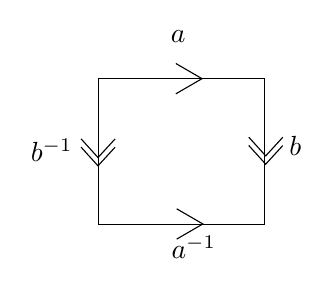
\begin{tikzpicture}[x=0.75pt,y=0.75pt,yscale=-1,xscale=1]
      %uncomment if require: \path (0,300); %set diagram left start at 0, and has height of 300
      
      %Flowchart: Process [id:dp4020928598077935] 
      \draw   (347.2,161.2) -- (427.2,161.2) -- (427.2,231.2) -- (347.2,231.2) -- cycle ;
      \draw   (355.12,190.12) -- (346.89,199.1) -- (338.72,190.08)(355.11,194.12) -- (346.88,203.1) -- (338.71,194.08) ;
      \draw   (435.92,189.32) -- (427.69,198.3) -- (419.52,189.28)(435.91,193.32) -- (427.68,202.3) -- (419.51,193.28) ;
      \draw   (384.4,153.8) -- (397,161.1) -- (384.4,168.4) ;
      \draw   (384.8,223.8) -- (397.4,231.1) -- (384.8,238.4) ;
      
      % Text Node
      \draw (380.73,136.8) node [anchor=north west][inner sep=0.75pt]    {$a$};
      % Text Node
      \draw (381.09,235.85) node [anchor=north west][inner sep=0.75pt]    {$a^{-1}$};
      % Text Node
      \draw (437.82,187.62) node [anchor=north west][inner sep=0.75pt]    {$b$};
      % Text Node
      \draw (313.27,188.71) node [anchor=north west][inner sep=0.75pt]    {$b^{-1}$};
      \end{tikzpicture} \]
  \end{center}
\end{itemize}

\vskip 0.5cm
[Write more stuff from images]

\vskip 0.5cm
\subsection*{n-Cells}
FOr $n \geq 1$, an $n$-cell is a topological space which is homeomorphic to an open $n-$dimensional ball. For $n = 0$, a $0-$cell is just a point.


\vskip 0.5cm
\subsection*{Cell Complex}
\begin{mathdefinitionbox}{}
  A cell complex is a topological space which is a disjonit union of cells of various dimensions.
\end{mathdefinitionbox}

\begin{mathdefinitionbox}{CW Complex}
  \vskip 0.5cm
  Write later
\end{mathdefinitionbox}

\begin{mathdefinitionbox}{Euler Characteristic}
  \vskip 0.25cm
  Write later
\end{mathdefinitionbox}

\subsection*{Next Time}
We'll begin studying \emph{\textbf{Algebraic Topology}}. We'll study different types of complexes.

\pagebreak

\section{Feburary 8 - Starting off with Algebraic Toplogy!}

\vskip 0.5cm
\subsection{Recap of the past}

\vskip 0.5cm
\begin{itemize}
  \item So far, we've seen Linear Algebra, Group Theory, and Point-set Topology with their main objects of study being Vector Spaces + Linear Transformations, Groups + Group Homomorphisms, and finally Topological Spaces + Homeomorphisms.
  \item We studied some important properties of Topological Spaces such as \textbf{openness and closedness, compactness and continuity.}
\end{itemize}

\subsection{Alg. Top. At. Last.}

\subsubsection*{Preview of the future}
Skipping ahead real quick, let's see where the topology we're going to develop shows up in physics and \emph{why} it's useful.

\begin{dottedbox}
  \emph{\textbf{Quantum Hall Effect:}} 
  \begin{itemize}
    \item Explain the effect later.
    \item It turns out that $\frac{ve^2}{h}$ is a \emph{topological invariant} of the many-body wavefunction. 
    \item In fact, this is a special case of \emph{Topologcal Band Theory}.
    \item In 2017, it was realized that $\approx 27 \%$ of our known materials have Topological bands!
  \end{itemize}
\end{dottedbox}

\begin{dottedbox}
  \emph{\textbf{Topological Phases of Matter:}} 
  \begin{itemize}
    \item Could be used for Topological Quantum Computing.
    \item Their classification is still an open problem.
  \end{itemize}
\end{dottedbox}

\begin{dottedbox}
  \emph{\textbf{Quantum Field Theory:}} 
  \begin{itemize}
    \item Any kind of non-perturbative niformation we can gain about our QFT's is valuable, and so Topologcial Invariants are valuable.
    \item Further, there is the focused branch \emph{Topological Quantum Field Theory} [write more later]
  \end{itemize}
\end{dottedbox}
\begin{dottedbox}
  \emph{\textbf{Why do there only exist fermions and bosons?}} 
  \begin{itemize}
    \item We'll cover this next week!
  \end{itemize}
\end{dottedbox}



\subsection{Topological Invariants}
A \emph{\textbf{Topological Invariant}} is a property of a space which remains unchanged (or invariant) up to Homeomorphism. That is, it does not change as long as we only continuously deform our space.

\begin{mathdefinitionbox}{}
  A homeomorphism $f$ is a continuous map between topological spaces $f : X \rightarrow Y$ such that $f \circ g = \mathrm{id}_Y$ and $g \circ f = \mathrm{id}_YX$
\end{mathdefinitionbox}

\vskip 0.25cm
Why are we even interested in Topological Invariants? Well, to show that two spaces $X, Y$ are homeomorphic we have to \emph{find} a homeomorphism between them. But how do we show that two spaces are \emph{\textbf{not}} homeomorphic? 

\vskip 0.25cm
We can't sit and verify \emph{every} map between the spaces. So, instead, we find some topologcal nivarant and show that the invarant differs for the two spaces!

\vskip 0.25cm
The issue is that the challenge of finding \emph{all topological invariants} is essentially intractible. It's simply too hard! So, instead, we weaken the condition. Rather than consider spaces up to Homeomorphism, we consider them \emph{up to homotopy}.

\begin{mathdefinitionbox}{Homotopy between Functions}
  \vskip 0.25cm
  \begin{itemize}
    \item We say there exists a Homotopy between continuous functions $f, g : X \rightarrow Y$ if there exsts a continuous map $H : X \times [0,1] \rightarrow Y$ such that $H(x, 0) = f(x)$ and $H(x, 1) = g(x)$.
    \item We denote this as 
    \[ f \sim g \]
  \end{itemize}
\end{mathdefinitionbox}

\begin{mathdefinitionbox}{Homotopy Equivalence}
  \begin{itemize}
    \item Two spaces are homotopy equivalent if
    \item Gven example of Circle and Cylinder
  \end{itemize}
\end{mathdefinitionbox}


\vskip 1cm
\subsection{Fundamental Group}

\vskip 0.25cm
This is the first topological invariant we'll study. It gives us a way to classfy all the possible \emph{paths} on a space.

\begin{mathdefinitionbox}{Paths}
  \begin{itemize}
    \item A \emph{\textbf{Path}} on a space $X$ is a map $\alpha : I \rightarrow X$ where $I = [0, 1]$. We say the path starts at $x_0$ and ends at $x_1$ if $\alpha(0) = x_0$ and $\alpha(1) = x_1$.
    \item A \emph{\textbf{loop}} is a path such that $\alpha(0) = \alpha(1)$.
    \item A constant path is a path of the form $\alpha(t) = x_0$ for all $t \in I$.
  \end{itemize}
\end{mathdefinitionbox}

\vskip 0.25cm
Further, we can define a sort of \emph{product} of two paths. We define the product as 

\begin{mathdefinitionbox}{Product of two paths}
  \[ \alpha \star \beta \defeq \begin{cases}
    \alpha(2s), \;s \leq 1/2 \\
    \alpha(2s+1), \;s > 1/2 \\
  \end{cases} \]
\end{mathdefinitionbox}

\vskip 0.25cm
Intuitively, this means we follow $\alpha$ for half of our time, and then $\beta$ for the remaining half of our time.

\vskip 0.25cm
\begin{mathdefinitionbox}{Inverse of a Loop} 
  \[ \alpha^{-1}(s) \defeq \alpha(1-s) \]
\end{mathdefinitionbox}

\vskip 0.25cm
Also, although gonig around a circle counterclockwise and then clockwise is not the same as just the constant map, we define an equivalence class on the set of paths such that $\alpha \sim \beta$ if the two paths are \emph{homotopic}. Under this relation, the two are the same.

\vskip 0.25cm
Notice that we have bilinear product, an identity loop, and an inverse for each loop. These are all the properties required of a group! So, we define the \emph{\textbf{Fundamental Group}} as the set of equivalence classes of paths

\begin{mathdefinitionbox}{Fundamental Group based at a point}
  The fundamental group of a space $X$ with basepoint $x_0$ is defined as 
  \[ \pi_1(X, x_0) = \{ [\alpha_{x_0}] \} \]
  with the product, inverse, and identity defined as above.

  \vskip 0.25cm
  \underline{Show later that the product is well defined!}
\end{mathdefinitionbox}

Notice that the fundamental group dependson the \emph{\textbf{base point}}. It turns out that if $X$ is simply-connected, then it \emph{doesn't matter which point we choose as the base!} The fundamental groups based at each point are Isomorphic.


\begin{dottedbox}
  \underline{Theorem:} If $f : X \rightarrow Y$ is a homotopy equivalence between topological spaces $X, Y$ then the fundamental groups of the spaces are isomorphic
  \[ \pi_1(X, x_0) \cong \pi_1(Y, f(x_0)) \]

  \vskip 0.5cm
  \underline{Prove later!}
\end{dottedbox}


\vskip 1cm
\subsubsection{Fundamental Group of the Circle}
Now that we've defined the Fundamental Group, let's actually compute it!

\begin{dottedbox}
  Draw Image and write formal argument later.
  
  \vskip 0.5cm
  Intuitively, the \emph{number of windings} is the topological invariant here. So, 
  \[ \boxed{ \pi_1(S^1) = \mathbb{Z} } \]
\end{dottedbox}

\begin{dottedbox}
  Quick note: The number of windings is called the \emph{\textbf{degree of the map}}. Later, we'll see how the degree of a map is physically impact to Field Configurations.
\end{dottedbox}


\vskip 1cm
\subsection*{Deformation Retract}

\begin{mathdefinitionbox}{Deformation Retract}
  \begin{itemize}
    \item A subset $R \subseteq X$ of a toplogical space $X$ is said to be a \emph{\textbf{deformation retract of $X$}} if there exists a homotopy $H$ between $R$ and $X$ such that 
    \[ H(r, t) = H(r, 0) \]
    for all $r \in R$ and $t \in I$.
    \item $X$ is contractible if it deformaton retracts to a point $x_0 \in X$.
  \end{itemize}
\end{mathdefinitionbox}

\begin{dottedbox}
  Note that if $X$ is a contractible space and deformation retracts to $x_0 \in X$, then 
  \[ \pi_1(X) \cong \pi_1(x_0) \cong \mathbf{1} \]
\end{dottedbox}

\vskip 0.5cm
\begin{dottedbox}
  \underline{Theorem:} 
  \[ \pi_1(x \times Y) \cong \pi_1(X) \oplus \pi_1(Y) \]
  where $\oplus$ denotes the direct product in additive notation.
\end{dottedbox}

\vskip 1cm
\subsection{Fundamental Group of a Torus}

Using the above theorem, we have 
\[ \pi_1(T) = \mathbb{Z} \oplus \mathbb{Z} \]

We also have the relation $ab a^-1 b^1 \sim 1$ which basically tells us that it is a commutative group $ab = ba$.

[Insert image]

\subsection{Fundamental Group of a Wedge Sum: $\mathbb{S}^1 \vee \mathbb{S}^1$}

[write this section later from image]

Note that in this case the fundamental group is not commutative.

\[ \pi_1(X, x_0)  = \mathbb{Z} * \mathbb{Z} \]

where $*$ denotes the free product.

\pagebreak
\section{February 13 - }


\vskip 0.5cm
\subsection*{Recap}
\begin{itemize}
  \item Write from picture.
  \item Write about different perspectives on $\mathbb{RP}^n$.
  \[ \pi_1 \left( \mathbb{RP}^2 \right) \cong \mathbb{Z}/2\mathbb{Z} \]
\end{itemize}

\vskip 0.5cm
The fundamental group is very simple to define, but it's generally very hard to compute. Further, there are spaces which which are \emph{not} homotopy equivalent but which the fundamental group \emph{cannot} tell apart. For instance, $\mathbb{S}^2$ and a single point both have trivial fundamental group.

\vskip 0.5cm
So, the fundamental group is simple but has some issues: notably, it kind of \emph{fails} at doing its job as an invariant. We will spend the next few weeks building more advanced invariants which become harder and harder to fool.

\vskip 0.5cm
\subsection{Lens spaces}

[write later]

\vskip 0.5cm
\subsection{Induced Homomorphisms}
If we have a map between topological spaces $f : X \rightarrow Y$ which is continuous at $x_0$, this map \emph{induces} a group homomorphism $f_* : \pi_1(X, x_0) \rightarrow \pi_1(Y, f(x_0))$ defined by 
\[ [\phi] \mapsto [f \circ \phi] \]

Let's verify that this map is well-defined. Consider two homotopic paths on $X$, $\psi \sim \psi$, for which there exists a homotopy $H$. Then, their images $f \circ \phi$ and $f \circ \psi$ are also homotopic with the homotopy $f \circ H$.

\begin{dottedbox}
  Note: 
  \begin{itemize}
    \item $(f \circ g)_{*} = f_* \circ g_*$ 
    \item $\mathbf{1}_* = \mathbf{1}$
  \end{itemize}
\end{dottedbox}

\subsubsection*{Some properties of Induced Homomorphisms}

\begin{itemize}
  \item $f$ is a homeomorphism $\implies$ $f_*$ is an isomorphism.
  \item $f$ is a homotopy equivalence $\implies$ $f_*$ is an isomorphism.
  \item $f$ is a retraction $\implies$ $f_*$ is an injective.
  \item $f$ is a deformation $\implies$ $f_*$ is an isomorphism.
\end{itemize}

\vskip 1cm
\subsection{Covering Spaces and Maps}

\begin{mathdefinitionbox}{}
  A covering space of $X$ is $(\tilde{X}, P)$ where $P : \tilde{X} \rightarrow X$ is such that 
  \begin{itemize}
    \item $P$ is surjective.
    \item $\forall x \in X$, there exxsts an open $U_x$ such that $p^{-1}(U_x)$ is 
    \[ \coprod U_{\alpha} \cong_{h} U_x \]
  \end{itemize}
\end{mathdefinitionbox}

For example, $R \rightarrow \mathbb{S}^1$, $\mathbb{S}^n \rightarrow \mathbb{RP}^n$.
[Write more about these].

\vskip 1cm
\subsection{CW Complexes}

\begin{itemize}
  \item CW Complexes are spaces built recursively by starting off with points, then adding lines, then planes, and so on\dots.
  
  \item Most surfaces we'll work with will be CW Complexes.
\end{itemize}

\begin{mathdefinitionbox}{$n-$cell}
   \vskip 0.25cm
   An $n-$
\end{mathdefinitionbox}

[Write later.]

\subsection{Limitations of the Fundamental Group}
\begin{itemize}
  \item $\pi_1$ is really sensitive to dimesnions $n \leq 2$, but fails to detect higher dimensional holes.
\end{itemize}

\subsection*{Add missing sections}

\subsection{Summary of Homotopy}

\pagebreak

\section{February 15 - Some Physics applications}

\vskip 1cm
\subsection{Outline for today}
\begin{itemize}
  \item What are phases of matter? Why are they interesting?
  \item Phase transitions, Landau Paradigm/Classification
  \item Examples of Homotopy defects
  \item Superfluidity/Mean Field Theory/Superconductivity
\end{itemize}

\vskip 1cm
\subsection{Phases of Matter}

\begin{itemize}
  \item In Condensed matter, we're concerned with systems with particles on the scale of Avogadros constant i.e. we're interested in \emph{macroscopic} behavior. It's impossible to study such systems by just solving Schrodinger's Equation.

  \item Further, there are some behaviors like Superconductivity which only arise in macroscopic settings.
  
  \item Consider a chain of $N$ individual electron spins for example. Insert image. The total hilbert space is the tensor product of the each spin hilbert space. 
  \item \[ \mathcal{H} = \otimes_n \mathcal{H}_i\]
  and has dimension $2^N$, which is huge!

  \item Furthermore, Condensed matter is usually only concerned with the states in a small corner of the total hilbert space. For example, only states at low temperatures.
  
  \item So, rather than studying the entire hilbert space, we partition it into \emph{phases}.
\end{itemize}

\subsubsection*{Transverse Ising Field}

Consdier the Hamiltonian 
\[ H = - \sum_{i = 1}^{N}  \left(\mathcal{Z}_{i} \otimes \mathcal{Z}_{i+1} + gX_i\right) \]

where 
\[ \mathcal{Z}_{i} = \begin{pmatrix}
  -1 & 0 \\
  0 & -1
\end{pmatrix}\;\;\;\; X_i= \begin{pmatrix}
  0 & 1 \\
  1 & 0
\end{pmatrix} \]
and $g$ is a \emph{tuning parameter} that we can control.

\begin{itemize}
  \item It turns out there are different phases associated with different ranges of values for the parameter $g$.
\end{itemize}

What do these two terms in the hamiltonian do?
The first term is basically a penalty for misaligned spins, and the second term just points in the $x_i$ direction.

\vskip 0.25cm
So, the frst guy wants spnis to be aligned, all pointing up or pointing down, whereas the second guy wants them to be pointing in some particular direction which might conflict with the spin up/down preferences of the first term.

\vskip 0.5cm
\underline{\textbf{\emph{$g = 0$:}}} In this case, the second guy is not present so our ground states are of the form 
\begin{align*}
  \ket{\psi} &= \ket{ \uparrow \uparrow \cdots \uparrow } \;\text{  or  } \\
  &= \ket{ \downarrow \downarrow \cdots \downarrow }
\end{align*}

\vskip 0.25cm
\underline{\textbf{\emph{$g = \infty$:}}} The solutions are of the form 

\[ \ket{\psi} = \ket{+} \otimes \ket{+} \cdots \ket{+} \]

where $\ket{+} = \frac{1}{\sqrt{2}} \cdot \left( \ket{\uparrow} + \ket{\downarrow} \right)$

\vskip 0.25cm
But notice that in the $g = 0$ case we have \emph{\textbf{2-dimensional ground state space}} whereas in the $g = \infty$ limit the groun state is a \emph{\textbf{1-dimensional space}}.

\vskip 0.5cm
This is actually a consequence of the simplest symmetry group $\mathbb{Z} / 2 \mathbb{Z}$!

\vskip 0.25cm
In physics, we call any operator which commutes with the hamiltonian as a \emph{Symmetry operator}. Such an operators has a common eigenbasis with the Hamiltonian so we can label the solution states using the symmetry group instead.

\vskip 0.5cm
The Transverse Field Ising Hamiltonian commutes with the operator\[ S = \Pi_i^{N X_i}\] and $S^1 = 1$ so $S$ has the same action as $\mathbb{Z} / 2\mathbb{Z}$ 

\vskip 0.5cm
If we act $S$ on the ground states of the $g = \infty$ case, they remain the same so we call these the \emph{symmetric} states. If we apply it to the states in the $g = 0$ space, then they flip so these are called the \emph{symmetrized} states.

\vskip 1cm
There is something called the \emph{\textbf{Order Parameter}} which tells us on average what the states look like. 

% \begin{mathdefinitionbox}{Order Parameter}
%   \[ \mean{m} = \frac{1}{N} \sum_{i = 1}^{N} \mean{\mathcal{Z}} \]
% \end{mathdefinitionbox}

\subsection{Heisenberg Hamiltonian and Symmetry Breaking}

\[ H = -J \sim_{i,j} S_i \cdot S_j = g \cdot \sum_{i} S_i \]

In this case, we can have \emph{\textbf{symmetry breaking}} from $SO(3) \rightarrow SO(2)$

\pagebreak

\section{February 20 - Homology and other fun stuff!}

Recall the Euler Characteristic, which was a topological invariant we came across a while ago, defined as 
\[ \chi(M) = \# V - \# E + \#F \]


It turns out that we can generalize this formula, for any CW-complex $M$, as 

\[ \boxed{\chi(M) = \sum_{n} (-1)^{n} \left(\# n\text{-cell}\right)} \]

\vskip 0.5cm
But we want to do better than this. So, we're going to \emph{\textbf{Categorify}} the Euler Characteristic!.

\vskip 0.5cm
Roughly, categorification entails replacing our invariant with a better invariant which has more information, and then go back to our original space using the \emph{\textbf{Forgetful functor}}.

\vskip 0.5cm
\[\begin{tikzcd}
	{\text{Invariant}} & {\text{Better Invariant}} \\
	{\text{Losing additional structure}} & {\text{More Information}}
	\arrow[from=1-1, to=1-2]
	\arrow[from=2-2, to=2-1]
\end{tikzcd}\]

\vskip 0.5cm
In this class, we will only discuss \emph{Simplicial Homology}, and Singular Homology if time permits. We're going to build Homology to be the \emph{better invariant} corresponding to the Euler Characteristic.

\begin{mathdefinitionbox}{Abelian Group}
  \vskip 0.25cm
  As a reminder, an \emph{\textbf{Abelian Group}} is a group $G$ whose elements commute: $gh = hg$ for all $g,h \in G$.
  \begin{itemize}
    \item For example, the cyclic groups $\mathbb{Z}/n \mathbb{Z}$ are all abelian groups.
    \item The rotations of a square form an abelian group.
  \end{itemize}
\end{mathdefinitionbox}

\vskip 0.5cm
An important \emph{type of element} of a group is one that can produce the rest of the group. For example, we can generate all of $\mathbb{Z}$ by repeated addition or subtraction of $1$. So, we say $\mathbb{Z}$ is generated by $1$.

\vskip 0.5cm
\begin{dottedbox}
  \emph{\textbf{Fundamental Theorem of Fintiely Generated Abelian Groups:}}

  \[ G = \underbrace{\mathbb{Z} \oplus \cdots \oplus \mathbb{Z}}_{\text{rank of }G} \;\;\oplus\;\; \mathbb{Z}/n\mathbb{Z} \oplus \cdots \oplus \mathbb{Z}/n\mathbb{Z} \;\; \oplus \cdots \]
\end{dottedbox}

\vsize 1cm
\subsection{Simplicial Homology}

\subsubsection*{Some definitions are in order}
To talk about Simplicial Homology, let's first define what a \emph{simplex} is:

\begin{mathdefinitionbox}{$n-$simplex}
\begin{itemize}
  \item   The $n-$simplex is defined to be the \emph{\textbf{oriented set}} 
  \[ \Delta^n = \{ \left(x_1, \cdots, x_n\right) \in \R^{n+1} \;|\; \sum_{i = 0}^{n} x_i = 1, x_i \geq 0 \} \] 

  \item These are basically generalizations of triangles to arbitrary dimensions.
\end{itemize}
\end{mathdefinitionbox}

[Include some figures.]

\vskip 0.5cm
Also, $[v_0, \dots, v_n]$ denotes the $n$-simplex $\Delta^n$ which has vertices $v_1, \dots, v_n$ and $[v_0, \hat{v}_i,\dots, v_n]$ denotes the simplex where the $i^{th}$ vertex is deleted from $[v_0, v^i, \dots, v_n]$. The symbol $\partial \Delta^n$ denotes the union of all faces i.e. the \emph{\textbf{boundary}} of the simplex.

\vskip 0.5cm
[Insert fgure]

\vskip 0.5cm
\subsection*{$\Delta$ structure on $X$}

\vskip 0.5cm
\begin{mathdefinitionbox}{}
  We can endow a space $X$ with$\Delta$-complex structure by defining a set of maps $\sigma_{\alpha} : \Delta^n \rightarrow X$ 
  \begin{itemize}
    \item 
  \end{itemize}
\end{mathdefinitionbox}

\vskip 0.5cm
For example, the Torus is a $\Delta$-complex structure formed by [write later]

\vskip 0.5cm
Note that the triangle with cyclic orientation is \emph{not} a $\Delta$-structure, but we can turn it into one as follows:

\vskip 0.5cm
[Insert figure]

\vskip 0.5cm
We \emph{define} a Homology on a $\Delta^n$ structure using an $n-$chain.

\begin{mathdefinitionbox}{n-chains}
  An $n-$chain on a space $X$ with delta structure $\Delta^n$ is denoted as $\Delta^n(X)$ and is the \emph{\textbf{Free Abelian Group}} generated by $\{e^n_{\alpha}\}$. Its elements look like arbitrary linear combinations
  \[ \sum n_{\alpha} e^n_{\alpha} \]
\end{mathdefinitionbox}

\subsubsection*{Boundary Map $\partial$}

\vskip 0.5cm
[Write more crap after class]

\vskip 0.5cm
\begin{dottedbox}
  \emph{\textbf{Lemma:}} $\partial_{n-1} \circ \partial_{n} = 0$ in the sequence
  \[  \Delta_{n-1}(X) \xrightarrow{\partial_{n-1}} \Delta_n(X) \xrightarrow{\partial_n} \Delta_{n+1}(X) \xrightarrow{\partial_{n+1}} \cdots   \]
\end{dottedbox}

\vskip 0.5cm 
\emph{\textbf{Proof:}} Write up after class.

\vskip 0.5cm 
Intuitively, this makes sense. The Boundary of a boundary is empty.

\vskip 0.5cm 
Another way to express this fact is to say that 
\[ \boxed{\text{Im}\left(\partial_{n+1}\right) \subseteq \ker\left(\partial_n\right) } \]

\vskip 0.5cm
Finally, we define the \emph{Simplicial Homology Group, $H_n^{\Delta}(X)$}  as 

\begin{mathdefinitionbox}{}
  \[ H_n^{\Delta}(X) = \ker \partial_n / \text{Im} \partial_{n+1} \] 
\end{mathdefinitionbox}

\vskip 0.5cm
The Homology Group counts the number of "holes" in the space $X$ [Explain the intuition for this with pictures later].

\vskip 0.5cm
\underline{Example:} Homology group of $\mathbb{S}^1$

\vskip 0.25cm
[Write later]

\vskip 0.25cm
[Insert image]

\[ \boxed{H_1(\mathbb{S}^1) = \mathbb{Z}}\]

\vskip 0.5cm 
\begin{dottedbox}
  \emph{Note:} \[ H_0(X) \]
  doesn't tell us much for path connected spaces $X$. [write more about this]
\end{dottedbox}

\vskip 0.5cm
\underline{Homology Group of a Torus}

\vskip 0.5cm
Writelater


\vskip 1cm
\subsection{Some useful homology calculations}
\begin{enumerate}
  \item $H_n(\mathbb{S}^n) = \mathbb{Z}$
  \item $H_1\left(\mathbb{RP}^n\right) = \mathbb{Z}/2\mathbb{Z}$
\end{enumerate}

\vskip 1cm
\subsection{Some properties of Homology Groups}

\vskip 0.5cm 
Since we want Homology to be a topological invariant, we require it to satisfy some properties. For instance, the Homology Group must not depend on the specific $\Delta$0structure we endow on the space.

\vskip 1cm 
\subsection*{Relation between $\pi_1$ and $H_1$}

It turns out (there's a theorem proving this) that the First Homology group is the \emph{\textbf{abelianization}} of the Fundamental Group. i.e.
\[ \pi_1(X) /\{ghg^{-1} = g\} \cong H_1(X) \]

\vskip 1cm 
\subsubsection*{First Homology group of the wedge-sum of two circles}
Calculate later.

\vskip 1cm 
The first homotopy and homology groups are very simply related as above. The higher groups have more complicated relations, but there do exist maps between the higher groups (for all orders?).

\pagebreak

\section*{February 22 - Applications of Homology}

\vskip 0.5cm
\subsection*{Recap}
\begin{itemize}
  \item Last time, we saw that the Homology groups of the torus are given by 
  \[ H_n\left( T^2 \right) = \begin{cases}
    \mathbb{Z} \oplus \mathbb{Z}, n = 1 \\
    \mathbb{Z}, n = 2, 0 \\
    0, \text{ else}
  \end{cases} \]
\end{itemize}

\vskip 0.5cm
Let's calculate the Homology groups of the sphere now. 

\vskip 0.5cm
\subsection{Homology of $\mathbb{S}^n$}

\vskip 0.5cm
We can endow $\mathbb{S}^n$ with the $\Delta$ complex consisting of two $n$-simplices and the simplex group is 
\[ \Delta_n \left(\mathbb{S}^n\right) = \mathbb{Z}\{U\} \oplus \mathbb{Z}\{L\}  \]

With 
\[ \ker \]
[Finish from picture]

\vskip 0.5cm
Let's do one more calculation.

\vskip 1cm
\subsection{Homology of $\mathbb{RP}^2$}

\vskip 0.5cm
The Planar Diagram of $\mathbb{RP}^2$ is as below, where $U$ and $L$ are the 2-simplices, $(a, b, c)$ are the 1-simplices $v$ and $w$ are the 1-simplices. The black arrows denote the gluing, whereas the blue arrows denote the simplex orientations.

\begin{center}
  \includegraphics*[scale=0.50]{Homology of RP2.png}
\end{center}

\vskip 0.5cm
[Write more from picture]

\vskip 1cm
\subsection{Formal Properties of Homologies}

\vskip 0.5cm
We want to make sure that Homology is indeed a topological \emph{invariant}, and we will do so using \emph{Induced maps} (we came across these when studying homotopy invariance as well).

For homotopy, we defined the induced map $f_*$. For Homology, we will define $f_{\#}$.

\vskip 0.5cm
\begin{mathdefinitionbox}{}
  Rather than defining the map $F_{\#} : H_n(X) \rightarrow H_n(Y)$, we define a map on the level of chain groups 
  \[ f_{\#} : \Delta_n(X) \rightarrow \Delta_n(Y) \] to have the action \[ \sigma \mapsto f \circ \sigma \]
  where $f : X \rightarrow Y$ is a homeomorphism.
\end{mathdefinitionbox}

\vskip 0.5cm
This then gives us an mnduced map between the homology groups because of the following lemma:

\vskip 0.5cm
\begin{dottedbox}
  \emph{\textbf{Lemma:}} 
\end{dottedbox}

The Kernel and Image of a map $\partial_n$ are preserved under the action of $f_{\#}$, thus so is their kernel (the homology group).

\begin{dottedbox}
  Note: $f$ is a homotopy equivalence, thus $f_{\#}$ is an isomorphism.
\end{dottedbox}

\vskip 0.5cm
\subsection*{Degree of a map}

\vskip 0.5cm
In physics, often we are interested in maps from the $n-$Sphere to itself.

\vskip 0.5cm
Now, for any such map $f : \mathbb{S}^n \rightarrow \mathbb{S}^n$, the induced map is $f_{\#} : \underbrace{H_n(\mathbb{S}^n)}_{\mathbb{Z}} \rightarrow \underbrace{H_n(\mathbb{S}^n)}_{\mathbb{Z}}$. 

\vskip 0.5cm
But notice that any such map $\mathbb{Z} \rightarrow \mathbb{Z}$ can be characterized as just multiplying each integer by some other integer $m$. This number $m$ is called the \emph{\textbf{degree}} of the map:

\vskip 0.5cm
\subsubsection*{Some Properties of the degree}

\begin{itemize}
  \item $deg(\mathbf{1}) = 1$
  \item $deg(\mathbf{1}) = 1$
  \item $deg(\mathbf{f}) = 0$ if $f$ is not surjective
  \item The degree of the antipodal map is $(-1)^{n+1}$
\end{itemize}

\vskip 0.5cm
This will allow us to prove the \emph{\textbf{Hairy Ball Theorem}} for $\mathbb{S}^n$!

\vskip 0.5cm

\begin{dottedbox}
  \emph{\textbf{Hairy Ball Theorem:}} Write statement later.
\end{dottedbox}

\vskip 0.5cm
\emph{\textbf{Proof:}} Suppose $V(x)$ is a unit tangent vector field i.e. for all $x \in \mathbb{S}^b$ we have $x \perp V(x)$

\vskip 0.25cm
We can define a homotopy between the maps $\mathbf{x}$ and $\mathbf{v(x)}$. In particular, we can get a homotopy equivalence between $\mathbf{1}$ and $\mathbf{-1}$ as
\[ f(tx) =  \]

\vskip 0.5cm
[complete after class]

\vskip 1cm
\section{Identical Particles} (Based on work by Leinass and Myrrheim)
Now we come to a physical application of $\pi_1(X)$! 

\vskip 0.5cm
Let $X$ be the coordinate space or configuration space for a single particle. Then, for $n$ identical particles, we would naively assume the configuration space is $X \times \cdots \times X$, but this does not account for the fact that the $n$ particles are identical! 

\vskip 0.5cm
If we have a configuration $(x_1, x_2, \dots, x_n)$, swapping any pair of them makes no distance. So, the \emph{actual} configuration space is 
\[ X / S_n \]
where $S_n$ is the $n$-th permutation group. Physically, this is fine because $X^n / S_n$ is locally isomorphic to $X^n$.

\vskip 0.5cm
Any configuration/path in $X^n / S_n$ can be \emph{lifted} to a number of configurations/paths in $X^n$ -- and this is what we do in Classicaly Mechanics! We choose only of the paths in $X^n$ and work in its locality. More formally, $X^n / S_n$ is a covering space for $X^n$.

\vskip 0.5cm
However, this doesn't work in Quantum Mechanics.

\vskip 0.5cm
Dealing with $S_n$ is annoying so let's just consider two particles for now, with $X = \R^n$. Then, the configuration space -- when using generalzed radial coordinates -- is 
\[ \left(\underbrace{\R^n}_{C.O.M.} \times \underbrace{\R_+}_{radial length} \times \underbrace{\mathbb{S}^{n-1}}_{rel. angular position}\right) / \left(\mathbb{Z}/2\mathbb{Z}\right) \]

And recall that $\mathbb{S}^{n-1} / \left(\mathbb{Z} / 2\mathbb{Z}\right)\cong \mathbb{RP}^{n-1}$. This is not a simply connected space, so $\pi_1\left(\mathbb{RP}^{n-1}\right)$ is nontrivial. Now, $\mathbb{S}^{n-1}$ is the universal covering space of $\mathbb{RP}^{n-1}$.

\vskip 0.5cm
[Fill in some detail]

\vskip 0.5cm
When we quantize this system, the number of phases that the wavefunction can pick when we switch the two particles is given by 
\[ \pi_1(\mathbb{RP}^{n-1}) = \begin{cases}
  \mathbb{Z}, n = 2 \\
  \mathbb{Z} / 2 \mathbb{Z}, n \neq 2 \\
\end{cases} \]

\vskip 0.5cm
This measn that in 3-dimensions, we can only have two types of particles (bosons and fermions!) but in \emph{\textbf{two dimensions}}, the phase can be \emph{any} value. Thus, these particles are called \emph{\textbf{anyons}}!

\vskip 0.5cm
\begin{dottedbox}
  \emph{Note:} The correct way of talking about this situation is in terms of \emph{vector bundles} because the wavefunction is actually a vector bundle defined over the configuration space.
\end{dottedbox}

\end{document} 

